%% @file main.tex
%% @title Orange: Recommendation Engine Report
%% @author Justin J. Wang
%% @date 4/26/17

%% bare_jrnl.ftex
%% V1.3
%% 2007/01/11
%% by Michael Shell
%% see http://www.michaelshell.org/
%% for current contact information.

%%*************************************************************************
%% Legal Notice:
%% This code is offered as-is without any warranty either expressed or
%% implied; without even the implied warranty of MERCHANTABILITY or
%% FITNESS FOR A PARTICULAR PURPOSE! 
%% User assumes all risk.
%% In no event shall IEEE or any contributor to this code be liable for
%% any damages or losses, including, but not limited to, incidental,
%% consequential, or any other damages, resulting from the use or misuse
%% of any information contained here.
%%
%% All comments are the opinions of their respective authors and are not
%% necessarily endorsed by the IEEE.
%%
%% This work is distributed under the LaTeX Project Public License (LPPL)
%% ( http://www.latex-project.org/ ) version 1.3, and may be freely used,
%% distributed and modified. A copy of the LPPL, version 1.3, is included
%% in the base LaTeX documentation of all distributions of LaTeX released
%% 2003/12/01 or later.
%% Retain all contribution notices and credits.
%% ** Modified files should be clearly indicated as such, including  **
%% ** renaming them and changing author support contact information. **
%%
%% File list of work: IEEEtran.cls, IEEEtran_HOWTO.pdf, bare_adv.tex,
%%                    bare_conf.tex, bare_jrnl.tex, bare_jrnl_compsoc.tex
%%*************************************************************************
\documentclass[12pt,journal]{IEEEtran} 
\usepackage{blindtext}
\usepackage{graphicx}
\usepackage{url}
\usepackage{algorithmic}
\usepackage{hyperref}
\usepackage{listings}

% *** GRAPHICS RELATED PACKAGES ***
%
\ifCLASSINFOpdf
  % \usepackage[pdftex]{graphicx}
  % declare the path(s) where your graphic files are
  % \graphicspath{{../pdf/}{../jpeg/}}
  % and their extensions so you won't have to specify these with
  % every instance of \includegraphics
  % \DeclareGraphicsExtensions{.pdf,.jpeg,.png}
\else
  % or other class option (dvipsone, dvipdf, if not using dvips). graphicx
  % will default to the driver specified in the system graphics.cfg if no
  % driver is specified.
  % \usepackage[dvips]{graphicx}
  % declare the path(s) where your graphic files are
  % \graphicspath{{../eps/}}
  % and their extensions so you won't have to specify these with
  % every instance of \includegraphics
  % \DeclareGraphicsExtensions{.eps}
\fi

% correct bad hyphenation here
\hyphenation{op-tical net-works semi-conduc-tor}


\begin{document}
%
% paper title

\title{Talent Analytic Studio: Recommendation Engine for Employee Training Courses at Orange - Silicon Valley}

\author{Justin~J.~Wang \footnotemark[*]

\thanks{author: Justin J. Wang, linkedin.com/in/justw, github.com/justwjr, phone: (626) 298-4825, email: justwjr@ucla.edu}% <-this % stops a space
\thanks{Orange - Silicon Valley, 60 Spear St, San Francisco, CA 94105}% <-this % stops a space
\thanks{University of New Haven(San Francisco), 44 Tehama St., San Francisco, CA 94105}}

% The paper headers
\markboth{\LaTeX\ - Journal of Data Science,~Vol.~6, No.~12, April~2017}%
{Shell \MakeLowercase{\textit{et al.}}: Bare Demo of IEEEtran.cls for Journals}

% make the title area
\maketitle

\begin{center}
     April 26, 2017
%  DRAFT
\end{center}

\begin{abstract}
%\boldmath
This paper describes implementing a hybrid collaborative filtering and content-based recommender based on the correlated cross-occurrence algorithm (CCO) to recommend courses for employees.  The performance of the recommendation engine model was evaluated using cross validation and mean average precision at k.  These tests allowed comparisons among the predictive strenght of different inputs.  Orange has the ambition to create a new learning experience through a Learning Management System.  The goal of Orange's employee training recommendation system is to advance the skillset of the company's workforce by promoting active participation and progress in completing SkillSoft courses.  The Talent Analytic Studio project leverages machine learning and analytics to solve HR challenges--addressing skill gaps and empowering people to take on new projects.
\end{abstract}

\begin{IEEEkeywords}
Cross-Occurrence algorithm, doc2vec, precision@k, PredictionIO, Spark MLlib, hybrid recommender system, collaborative filtering, content-based recommendation engine\end{IEEEkeywords}

\IEEEpeerreviewmaketitle



\section{Introduction}

For this project, we used the CRISP-DM methodology, which stands for Cross Industry Standard Process for Data Mining, figure \ref{fig:crisp-dm}. This paper is structured with the CRISP-DM process model in mind.

\begin{figure}[htbp]
\begin{center}
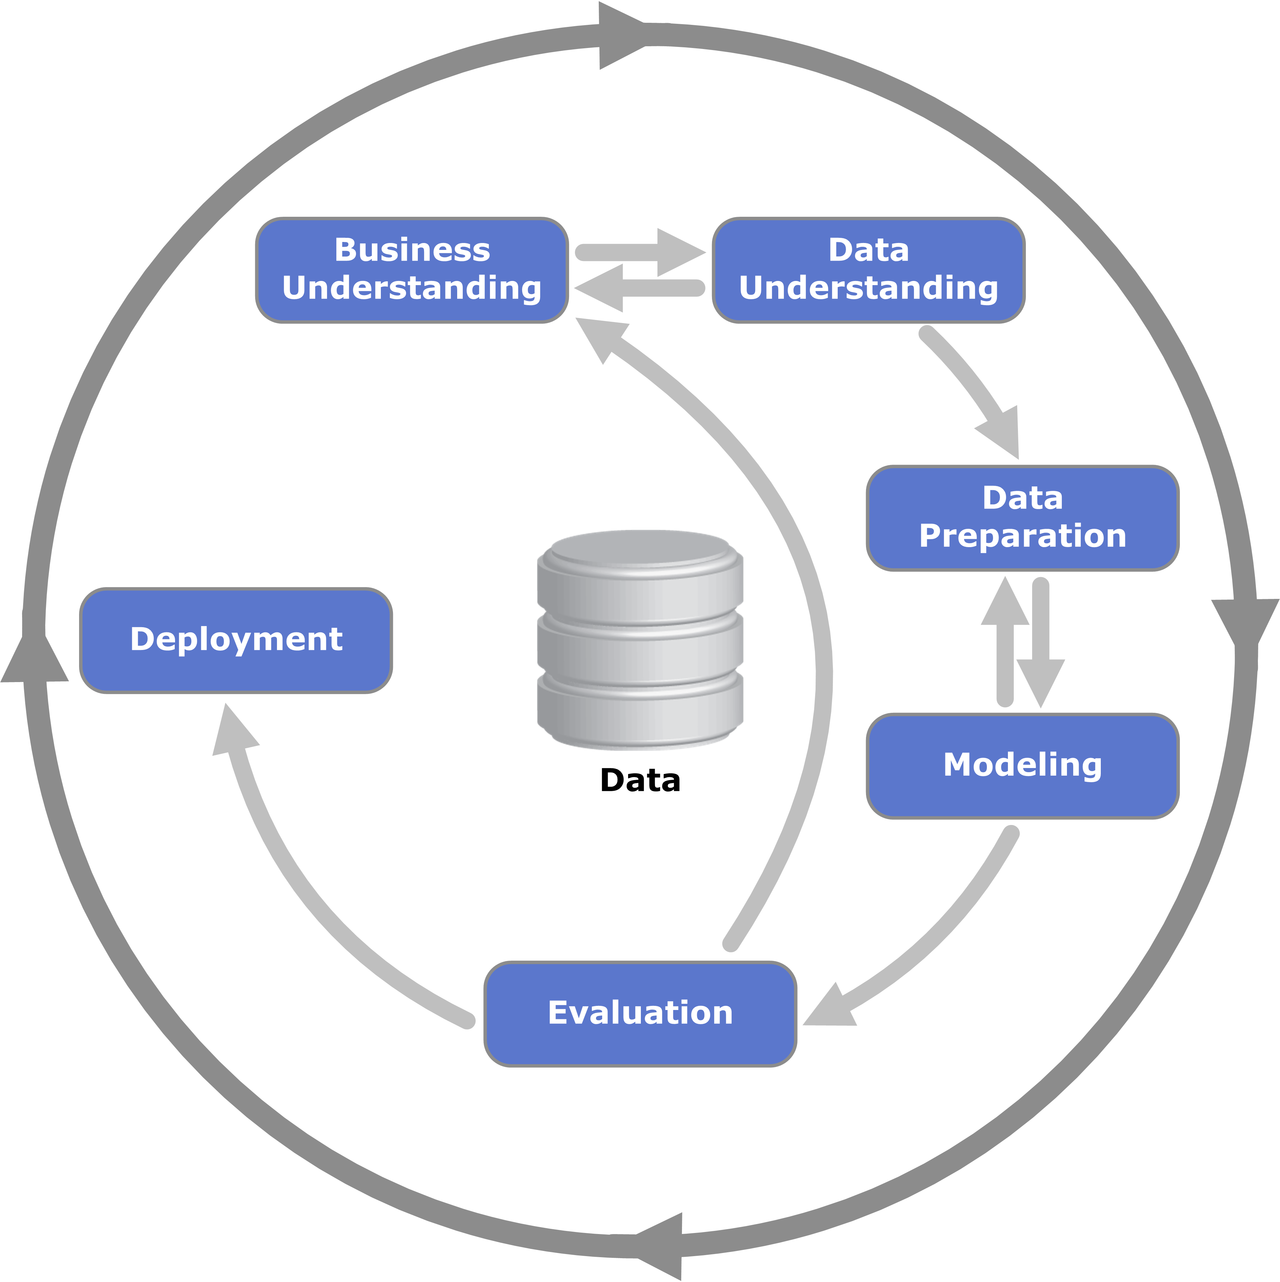
\includegraphics[width=1\columnwidth]{CRISP-DM_Process_Diagram}
\end{center}
\caption{CRISP-DM Process Diagram}
\label{fig:crisp-dm}
\end{figure}

\subsection{Business Understanding}

The point of implementing this internal recommender system for training courses is to get employees to actually take recommended course, in a way that betters the employee experience through personalization.  Orange is a multi-national corporation with all different types of employees.  The purpose recommending courses is also to address skill mismatch for govermenent or unionized employees to update their skillsets and move to new positions.

The desired outcomes and impacts are huge increase in employee training activity, retention, and completion rates; as well as engaged employees who produce higher quality work, offer diverse skillsets, and provide excellent customer experiences.

\subsection{Data Understanding: Datasets}

The datasets used by the recommendation engine comes from 3 sources: the SkillSoft catalog, which summarizes the offered courses; employee data, which comes from the profile and interactions within the Plazza social network; and the training record of past courses completed by employees.  Orange has over 155,000 employees as of December 31st, 2016  \cite{orangeSA}.  The pilot dataset consists of 500 users.  Figure \ref{fig:schema} illustrates the schema and tables of the relational database.

\begin{figure}[htbp]
\begin{center}
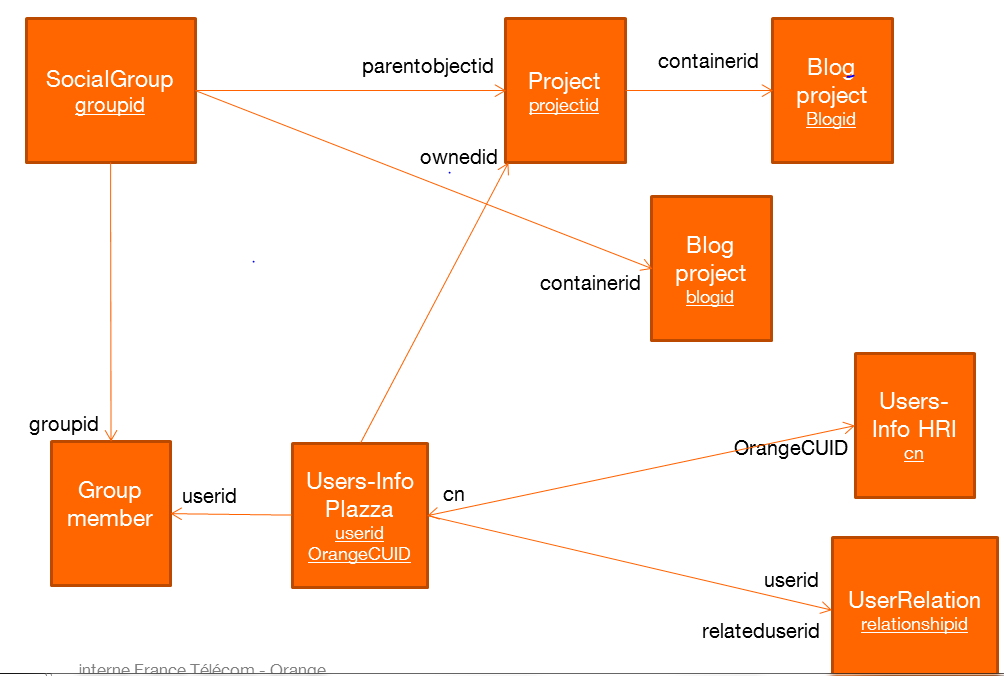
\includegraphics[width=1\columnwidth]{schema}
\end{center}
\caption{Database Architecture: Schema for User-related Tables}
\label{fig:schema}
\end{figure}

\subsection{Preparing and Ingesting the Data}

The StepIngestor.java program imports the data from relational tables to the EventServer.  We use the Amazon Report, Catalog, Group Member, Project, Social Group, Step, Training Update Catalog, User Info Plaza, and User Relation tables, covering a variety of different types of events.  After preparing and ingesting the data, we build the engine.  Figure \ref{fig:DistEventTypes} shows the distribution of the various types of events used in training the model.  Courses taken is the primary event.

\begin{figure}[htbp]
\begin{center}
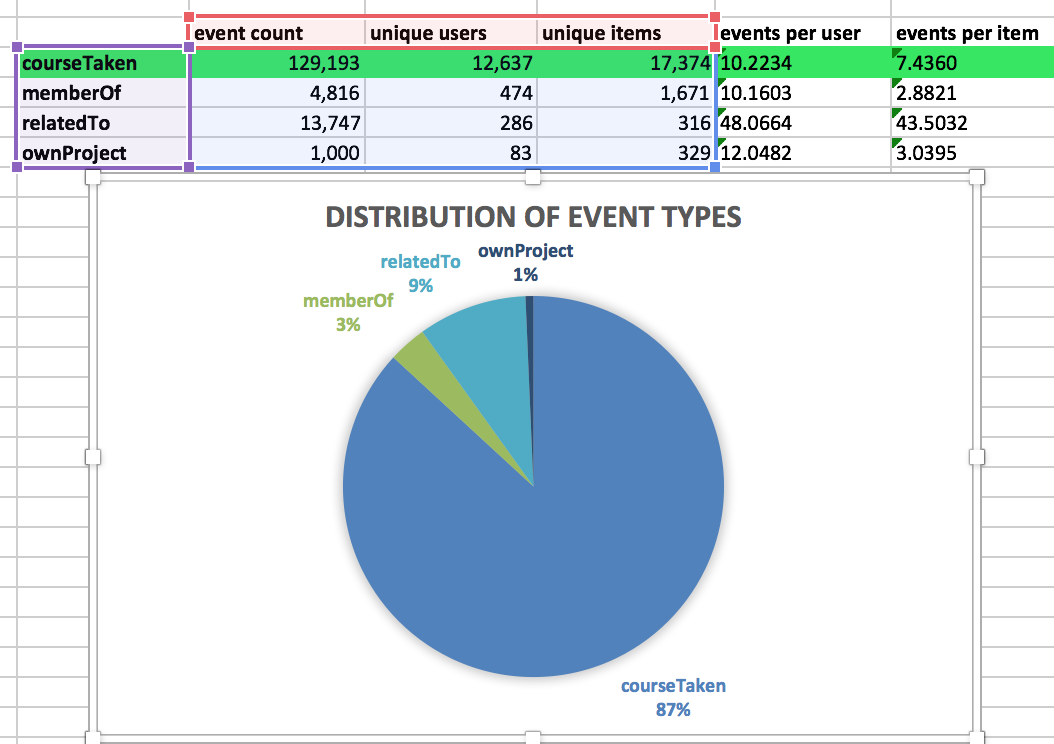
\includegraphics[width=1\columnwidth]{DistEventTypes}
\end{center}
\caption{Distribution of Various Event Types}
\label{fig:DistEventTypes}
\end{figure}

\subsection{Modeling}

Next, we train the model and deploy the engine on the server.  Once that is completed, we are able to send API requests for a user and receive recommendations.  For this task, we use cooccurrence recommenders with Spark.  The Universal Recommender engine template from PredictionIO lets us create a cutting edge recommender that is fast, scalable, extremely flexible for use in many different contexts, and can use almost any applicable data.  It uses Spark, Mahout, and a search engine \cite{patferrel}.  Figure \ref{fig:lambda_architecture} depicts the lambda architecture for the PredictionIO framework.

\begin{figure}[htbp]
\begin{center}
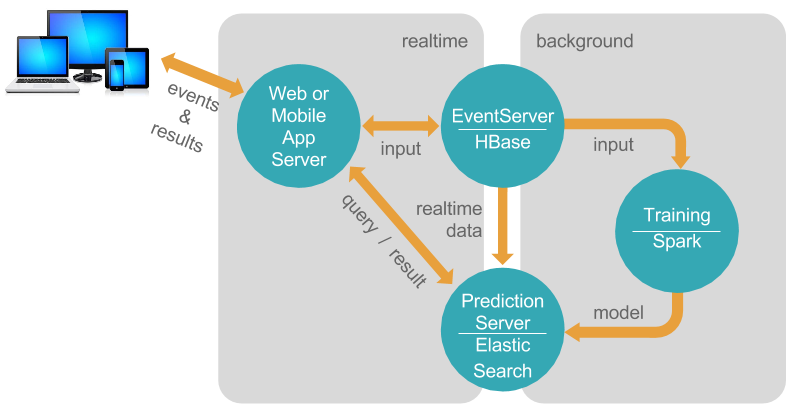
\includegraphics[width=1\columnwidth]{pio-architecture}
\end{center}
\caption{Lambda Architecture of the PredictionIO Framework}
\label{fig:lambda_architecture}
\end{figure}

Once deployed, the engine allows realtime input and queries.  Models re-train in the background and realtime data can be used in responding to queries.

\section{Why Correlated Cross-Occurrence Improves Upon Collaborative Filtering}

The correlated cross-occurrence algorithm auto-correlates different user actions to make better recommendations.  Pure collaborative filtering recommenders are based on the co-occurrence matrix, constructed as $C^tC$, where each row of $C$ represents a particular user, and each column represents a particular course.  The value in each cell entry in $P$ is the weighted preference for the corresponding user-course.  Entries in $C^tC$ are similarity scores between courses.  $C^tC$ compares column to column using a log-likelihood based correlation test, which has been shown to perform much better than cosine similarity because log-likelihood filters unimportant similarities \cite{patferrel}.  The cooccurrence matrix gets multiplied by a vector $h_c$ representing a user's history of the action, such as courses taken.  The result is the vector of recommendation scores: $r = (C^tC)h_c$.

Spark MLlib's implementation of collaborative filtering and Mahout's ALS recommender both use alternating least squares to perform matrix factorization to learn latent factors used to predict missing entries; however, the co-occurrence matrix is limited to only feedback that can be translated to the strength of user actions on items.  In contrast, the Universal Recommender's correlated cross-occurrence algorithm is able to ingest any number of user actions, events, profile data, and contextual information \cite{UniversalRecommender}.

To illustrate, the idea behind correlated cross-occurrence is that we can improve recommendations by incorporating more than 1 preference indicator by summing cross occurrences.  $e.g.$ to incorporate project team and social group, construct the cross occurrences, $(C^tP)h_p$ and $(C^tS)h_s$, respectively.  The approach is to find the most similar/like-minded users to a target user.  The final result is context-aware collaborative filtering: 

\begin{equation}
    r = (C^tC)h_c + (C^tP)h_p + (C^tS)h_s
\end{equation}

For our dataset, we have implicit feedback on finishing a course and not finishing, which we can map to number values related to the level of confidence in observed user preferences.  In our initial development, we did not differentiate between completing a course or not; taking a course maps to a score of 1.  If we had ratings data, that would be considered explicit feedback.  The contextual information from users that we ingest into the engine include social group, user relations, and work project.  Social group and user relations information come from the Plazza internal social network.  Events are logged when employees join a group or connect with colleagues.  We also feed in data on which work projects employees are part of, for example, I am part of project \#3256: Talent Analytic Studio.


\section{The Correlated Cross-Occurrence Algorithm}\cite{UniversalRecommender}

Correlated Cross-Occurrence \cite{Mahout}

\label{alg1}                           % and a label for \ref{} commands later in the document
\begin{algorithmic}                    % enter the algorithmic environment
    \REQUIRE spark-itemsimilarity to use multiple user actions
\RETURN recommendations favoring ones that have the stronger intrinsic indicators
\vspace{1px}
   \STATE $\enspace$ Mahout will use cross-action cooccurrence analysis to limit the views to ones that do predict purchases. We do this by treating the primary action (purchase) as data for the indicator matrix and use the secondary action (view) to calculate the cross-cooccurrence indicator matrix.

    $\enspace$ spark-itemsimilarity can read separate actions from separate files or from a mixed action log by filtering certain lines.
   
\end{algorithmic}

\begin{figure}[htbp]
\begin{center}
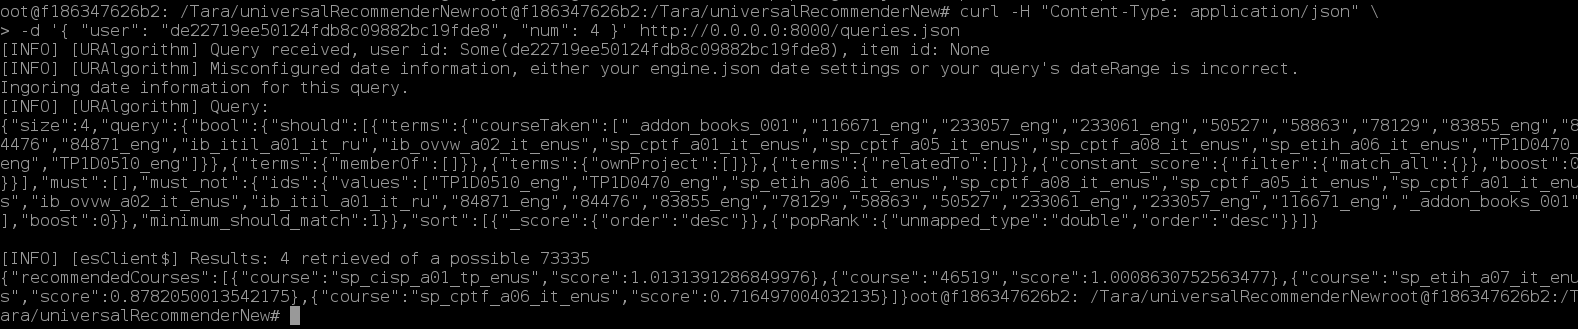
\includegraphics[width=1\columnwidth]{examplequeryforuser}
\end{center}
\caption{Example Query to Pull Top 4 Recommendations for a User}
\label{fig:example query for user}
\end{figure}

     \subsection{The Universal Recommender}
     
     The correlated cross-occurrence algorithm is a hybrid between collaborative filtering and a content-based recommender, supporting a wide variety of user input data to indicate tastes.  Apache Spark MLlib's Collaborative Filtering algorithm uses the alternating least squares algorithm to learn a small set of latent factors from a single type of user action represented in a weighted user-item association matrix.  Hence, pure collaborative filtering could construct a matrix based off courses taken, but not different types of events like joining a social group.  In contrast, the universal recommender's cross-occurrence algorithm (figure  \ref{fig:mahout_recommender_architecture}) can accept multiple different types of user events or contextual information and is arguably the only publicly documented recommender to do this.  It also supports item properties for filtering and boosting recommendations. \cite{UniversalRecommender}
     
     \begin{figure}[htbp]
    \begin{center}
    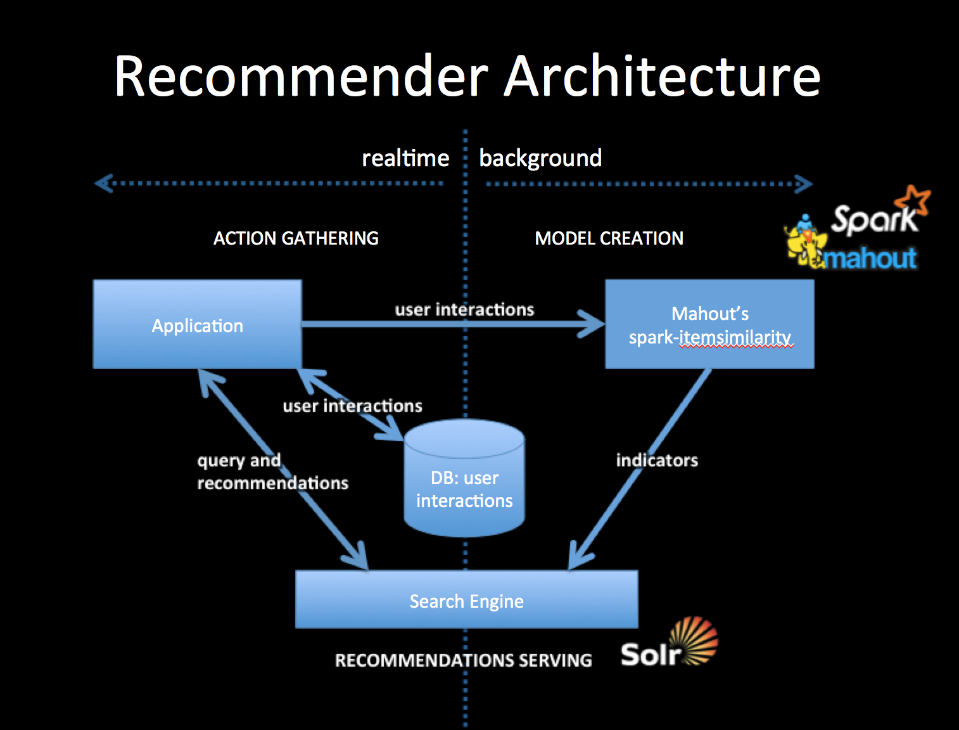
\includegraphics[width=1\columnwidth]{mahout_recommender_architecture}
    \end{center}
    \caption{Mahout Cooccurrence Recommender with Spark}
    \label{fig:mahout_recommender_architecture}
    \end{figure}


\subsection{Facing the Cold Start Problem}

Recommender engines based on user history have an inherent challenge in providing personalized recommendations for new users who have no historical data.  An engine trained only on past courses taken would be at a loss in recommending courses for an employee who has not yet taken any.  Our implementation addresses this issue by considering other event types, not only courses taken.  We have other context on user behavior such as being part of a work project or a member of a social group on the internal social network.  This solution for the cold start problem gracefully improves with more user history and as items have more interactions.  Almost all employees in the organization will quickly become part of a project or group.

Another answer to the cold start problem is a content-based approach, which would provide a solution for both new users with no history as well as new courses with too short a lifespan.  For instance, if we use intrinsic indicators from the courses such as the Series that the course belongs to, or if we construct indicators from the course descriptions, then similar items would get recommended.

Other possibilities include forcing new users to answer questions about their preferences or to simply start off with the most popular courses.

\subsection{Visibility Control}

The engine we are using has modifications to remove duplicate courses and ones for which the user has not satisfied the prerequisites.  It also filters items the user has already seen.  This logic gets implemented after all the scores are output by the engine.  The top 20 scoring courses minus omissions get shown to the user.  Currently, the plan for the front end is an email to the employee showing the personalized recommendations.  Figure \ref{fig:amazon_architecture} shows the architecture of the Reactor service.

 \begin{figure}[htbp]
\begin{center}
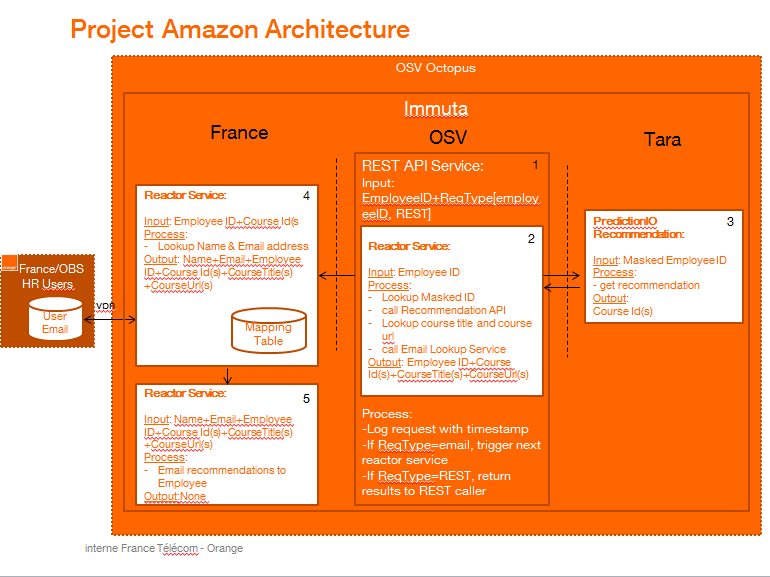
\includegraphics[width=1\columnwidth]{amazon_architecture}
\end{center}
\caption{Email Recommendations to Employees through Reactor Service}
\label{fig:amazon_architecture}
\end{figure}


\section{Evaluation Metrics}  \label{sec:Evaluation Metrics}
In this section, we discuss offline evaluation techniques for the recommender system.  Since the project is not yet in production, it is not possible to conduct experiments and run A/B testing, which would be the ideal way to evaluate algorithm variants to see how well changes improve meaningful metrics such as rate of course completion among a group of employees.  Instead, we turn to offline evaluation techniques, some of which are root-mean square error (RMSE), mean absolute error (MAE), mean average precision at k (MAP@k), and precision at k (precision@k), which measures the portion of relevant items amongst the first k items \cite{EvaluationExplained}.  MAP@k is the best metric to use because it takes into account the ordering of the recommendations, so that a model that shows good recommendations first scores higher.  RMSE and MAE are not good evaluations metrics to use because we care only about the top k recommendations, and the degree to which a particular predicted course is off from actual history is not a metric we could like to measure absolutely, since we are not using ratings data.  We use a rating threshold to define whether a recommendation is relevant, meaning a score above the threshold counts as relevant. \ref{fig:precision at k}

These offline, cross-validation testing methods are severly limited and some results are known to be contrary to real-world results discovered through A/B tests \cite{ActionMLAdvancedTuning}.  The solution is to run on-line experiments.  Increasing data used in training will almost always increase cross-validation test results, but randomizations and tuning for recency will almost always decrease scores.  This phenomenon is another example of how cross-validation tests for recommender systems conflict with real-world evaluation, since you would reason that more recent patterns in preferences would lead to better recommendations.

\begin{figure}[htbp]
\begin{center}
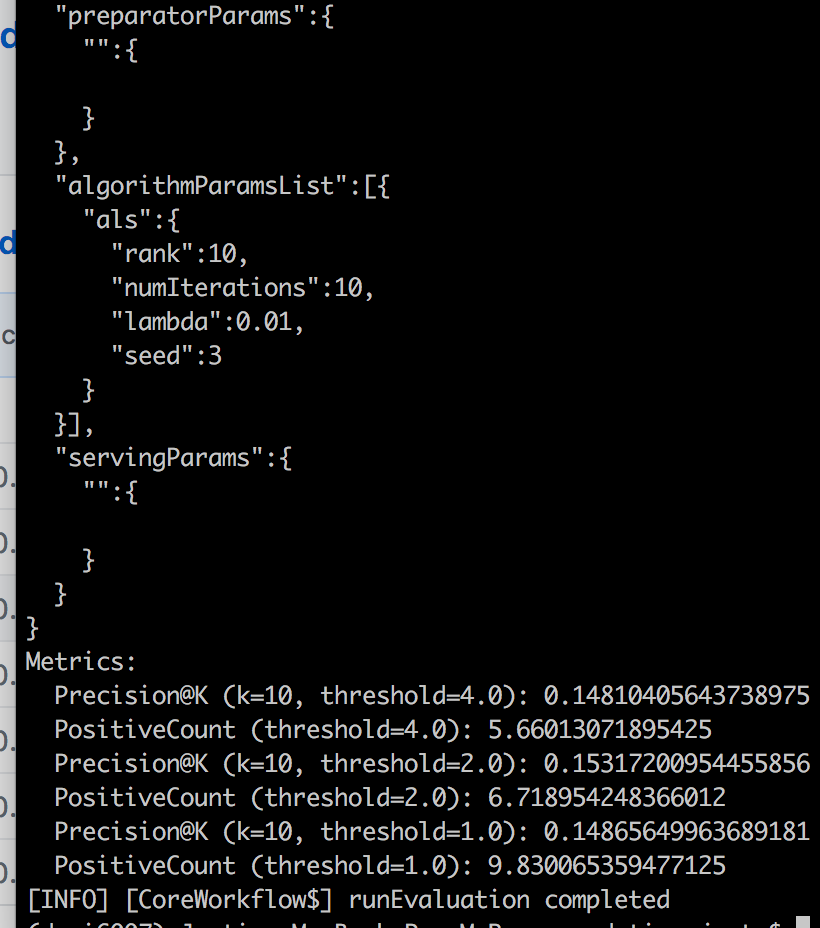
\includegraphics[width=1\columnwidth]{precision_at_k.png}
\end{center}
\caption{precision@k Evaluation Metric on the Recommendation Engine}
\label{fig:precision at k}
\end{figure}


Offline evaluation metrics, such as precision@k allows us to tune the engine to find optimal parameters.  For the training course recommendations, there are no user ratings for courses.  Currently the engine counts taking a course as an event.  Given more time for further development we could differentiate whether a person took a course, and whether or not the course was completed.  Hence, our event types would be either 1)"started and finished course" or 2)"started course but did not finish".


\subsection{Split the Data into Training and Testing Sets}
Once we have the data from the EventServer, we split the data into train and test sets (Figure \ref{fig:gottraintestsplitfiles}):

\begin{figure}[htbp]
\begin{center}
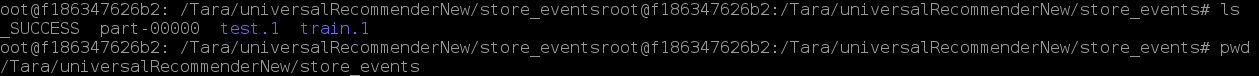
\includegraphics[width=1\columnwidth]{gottraintestsplitfiles}
\end{center}
\caption{Training and Testing Sets Stored in HDFS}
\label{fig:gottraintestsplitfiles}
\end{figure}

\subsection{MAP@k}

We ran cross-validation tests on the deployed UR using ActionML's analysis tools \cite{ActionMLAdvancedTuning}.  precision@k is the percentage of relevant courses among the first k recommendations.  Average precision introduces the notion that order matters, where score is higher if relevant recommendations are shown first.  The formula for average precision at n is:

\begin{equation}
ap@n = \frac{\sum_{k=1}^n P(k)}{min(m,n)} \!
\end{equation}

, where $m$ is the number of relevant courses and $n$ is the number of predicted courses.  If the denominator is zero, $P(k)/min(m,n)$ is set to zero. \cite{kaggleMAP}

Mean Average Precision at k (MAP@k) is the average of the average precision of each user:

\begin{equation}
MAP@k=\frac{\sum_{i=1}^N ap@k_i}{N}
\end{equation}
, where N is the number of users.

Contest submissions for recommendation engine challenges on Kaggle use MAP@k as the evaluation metric.

\subsection{Results Compared to Random Selection}

Figure \ref{fig:mapkResults} shows the mean average precision at values of k from 1 to 20.  At 20 recommendations, the model had a $map@k$ of 0.0928, which performed better than random sampling according to their distribution from the training set, which scored 0.0081.

\begin{figure}[htbp]
\begin{center}
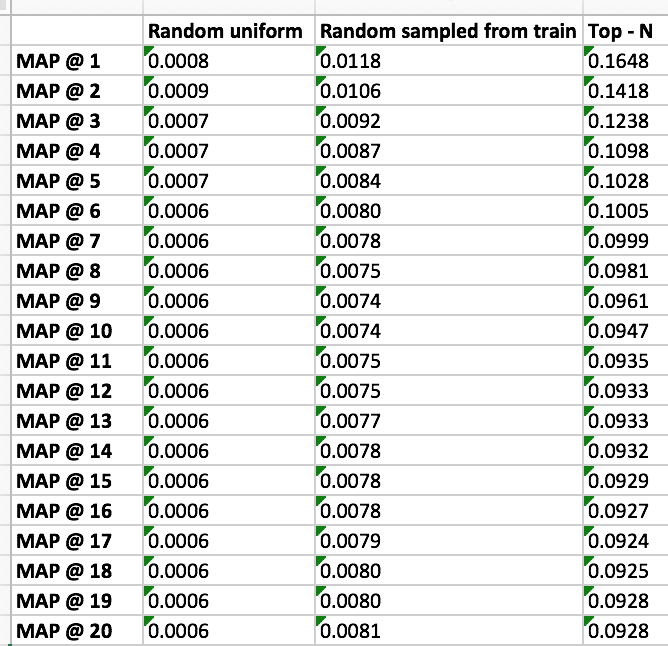
\includegraphics[width=1\columnwidth]{mapkResults}
\end{center}
\caption{MAP@k Results Compared to Random Samples}
\label{fig:mapkResults}
\end{figure}

The random uniform column draws a random sample uniformly from all items.

\begin{figure}[htbp]
\begin{center}
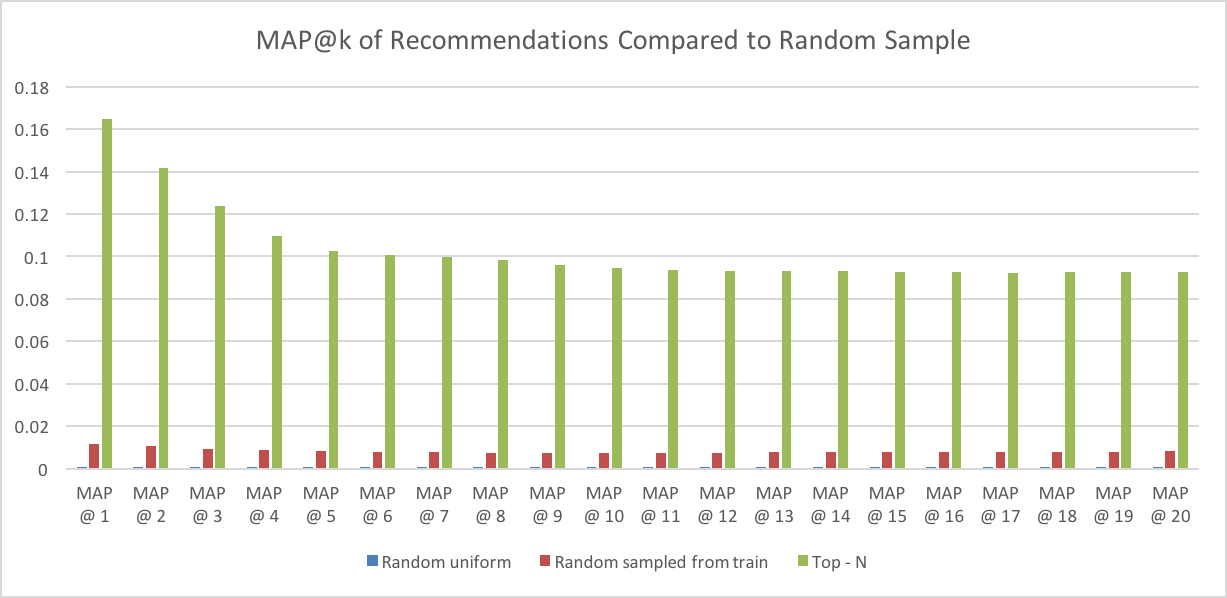
\includegraphics[width=1\columnwidth]{MAPkChart}
\end{center}
\caption{MAP@k Recommendations Compared to Random Samples}
\label{fig:mapkChart}
\end{figure}

 \cite{ActionMLAdvancedTuning}

\subsection{Discovering the Indicative Event Type}

We use cross validation testing to find the strongest indicators using the universal recommender's map@k tool for measuring the relative predictive strength of a given indicator type.  Then we would know the predictive strength of not finishing a course versus finishing a course.  Also, we could test how helpful Plazza network data is in making recommendations.  e.g. To what extent do users who join the same social group take the similar courses? \cite{ActionMLAdvancedTuning}

To compare the strength of the various secondary indicators, we ran MAP@k tests for each separate event (Figure \ref{fig:MAP_separate_indicators}):

\begin{figure}[htbp]
\begin{center}
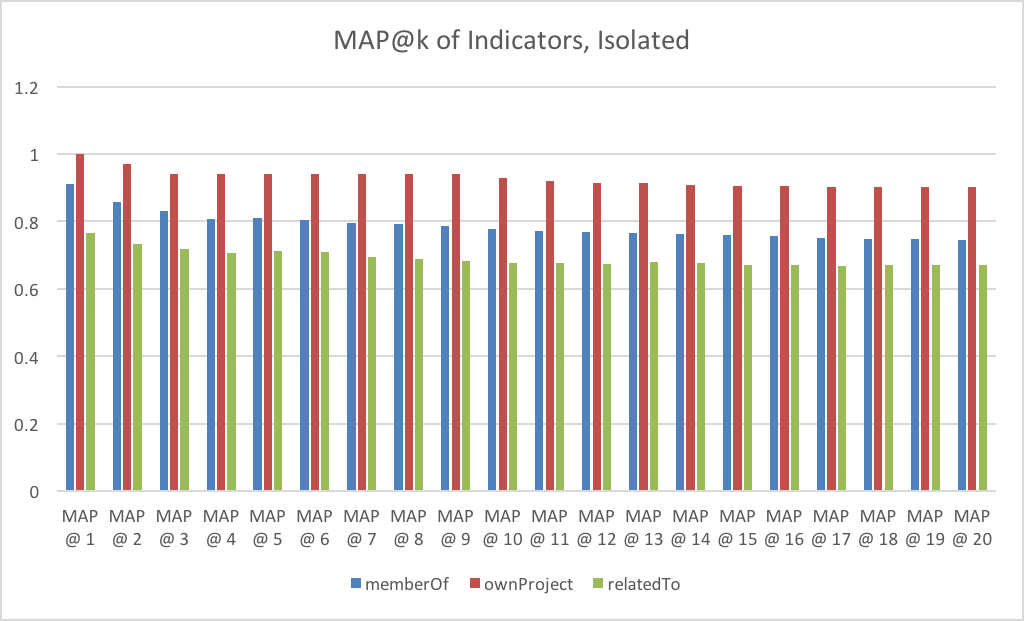
\includegraphics[width=1\columnwidth]{MAP_separate_indicators}
\end{center}
\caption{Comparing Predictive Strength of Secondary Indicators}
\label{fig:MAP_separate_indicators}
\end{figure}

We can see that belonging to a project is a stronger indicator that being a member a group (Figure \ref{fig:MAP_separate_indicators}).  Social relationships was the weakest indicator of the three event types.

\subsection{Deploying the Engine in Production}

  We use Apache PredictionIO (incubating),a full stack machine learning environment on top of Apache Spark, to deploy the recommendation engine as a web service in production.  It allows developers to iterate on production-deployable machine learning engines.  The infrastructure is open source, fast and scalable.  The tech stack includes Spark, MLlib, HBase, HDFS, Spray, Elasticsearch, Apache Mahout, Maven, Java, and Scala.  Spark is the default processing engine for PredictionIO.  Figure \ref{fig:URdataFlow2} shows the logical architecture and data flow for The Universal Recommender template.  We use internal servers to handle all the data storage and computing on premises.

\begin{figure}[htbp]
\begin{center}
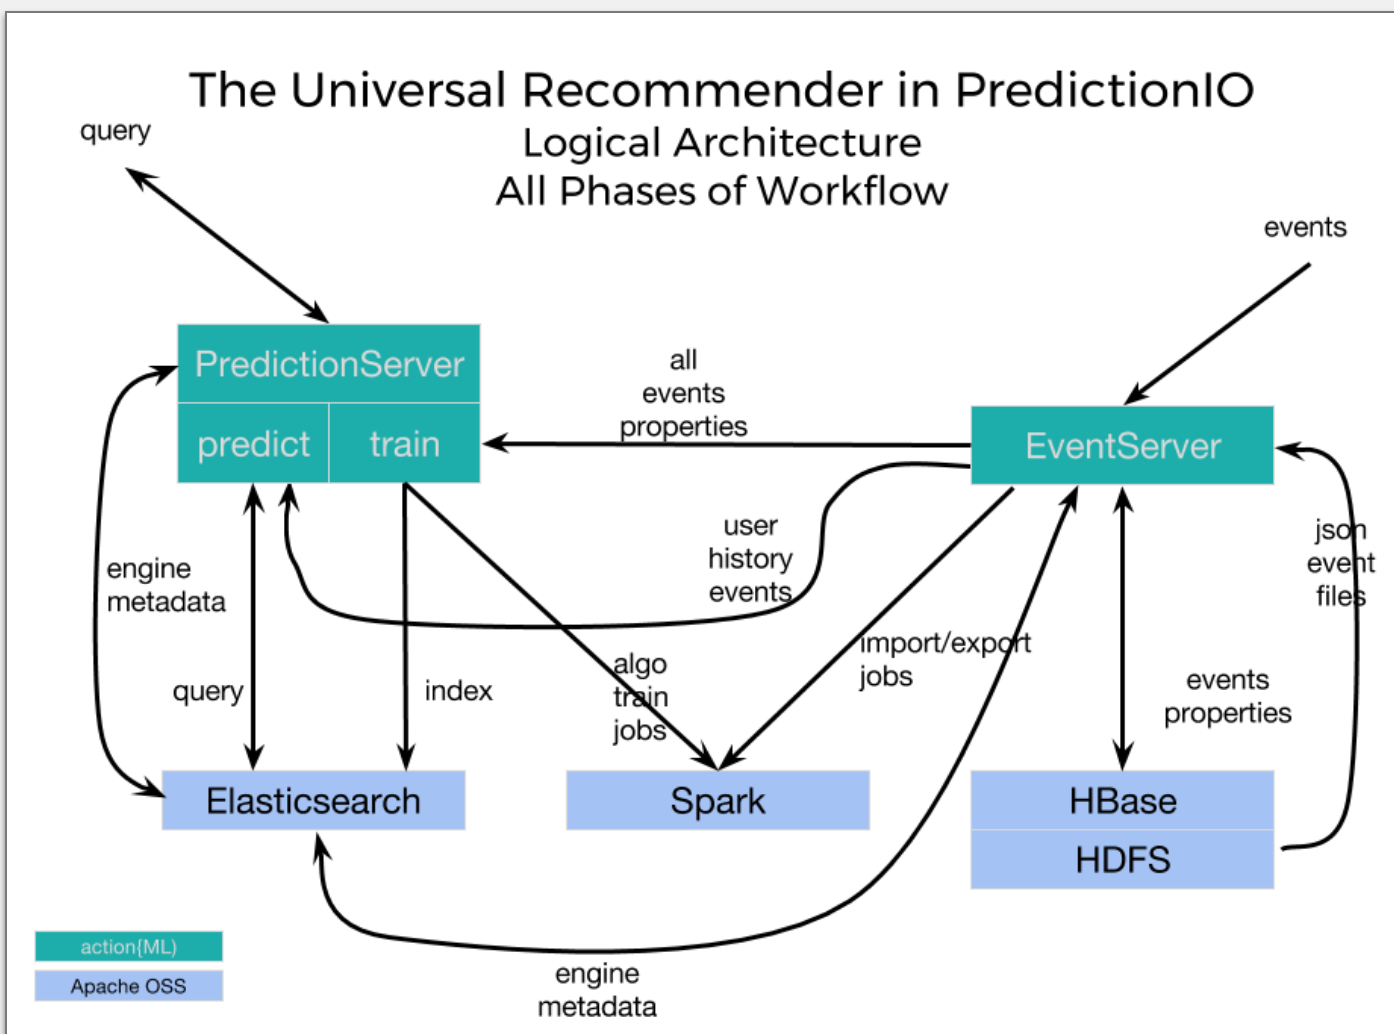
\includegraphics[width=1\columnwidth]{URDataFlow2}
\end{center}
\caption{Logical Architecture and Data Flow for UR}
\label{fig:URdataFlow2}
\end{figure}

The Universal Recommender requires Elasticsearch to be used as the storage backend for the meta data repository, which together with HBase, which is used as the backend of the event data repository, is generally faster than PostgreSQL and is able to host very large tables (billions of rows X millions of columns) atop clusters of commodity hardware.  \cite{UniversalRecommender}



%%%%%%%%%%%%%%%%%%%%%%%%%%%%%%%%%%%%%%%%%%%%%%%%
\hfill

\subsection{Adding Content Models}
Content models could be added to the correlated cross-occurrence model using latent direchlet allocation (LDA) to model topics from text given by course descriptions.  To start, we could try creating vectors using doc2vec check pairwise cosine similarities.

\subsection{Doc2Vec Experiment}
One of the challenges with working with this dataset is that the Skillsoft course catalog updates quarterly, where an updated course adopts a new course id.  The same course ends up having multiple different course ids, which messes up the recommender system, so we needed a way to identify which courses should be considered as the same course id.  A rudimentary approach is to fuzzy match on the course titles.  We used the python package called FuzzyWuzzy \cite{fuzzywuzzy}, which matches strings based on the Levenshtein distance to calculate the differences between sequences.  Partial results are shown in Figure \ref{fig:Levenshtein}.

%%%%%
\begin{figure}[htbp]
\begin{center}
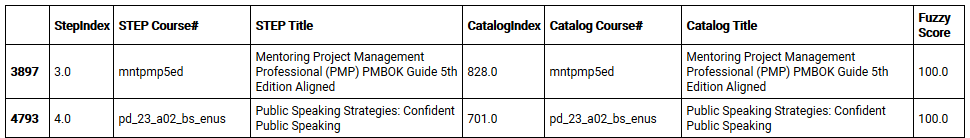
\includegraphics[width=1\columnwidth]{fuzzywuzzy_top}
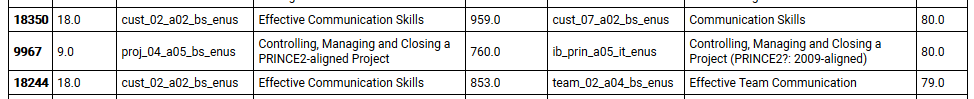
\includegraphics[width=1\columnwidth]{fuzzywuzzy_score_80}
\end{center}
\caption{Levenshtein Distance Between Course Titles}
\label{fig:Levenshtein}
\end{figure}
%%%%%%

  Obviously, when the fuzzy score between two titles is 100\%, we can confidently determine that they're the same course.  For results that were not a perfect match, it may be tempting to choose a threshold score and say that match scores above 80\% lets us group the two courses together; however, this rule would result in erroneous determinations.  For example, we observed in the catalog, one course named "Black-Box Software Testing Techniques", and another course named "White-Box Software Testing Techniques", completely different courses whose titles differ by one word, resulting in a fuzzy match score of 86\%.  Matching course titles based off anything other than a perfect match becomes problematic.  For instance, the prime offender to this approach are the two courses: "TestPrep 1Z0-808 Java SE 8 Programmer I", and "TestPrep 1Z0-809 Java SE 8 Programmer II", whose fuzzy match score is 97\%.  Title alone would not give us an automated way to find updates unless there is an exact match.

A semantic approach using Gensim's doc2vec \cite{rehurek_lrec} on course descriptions is an interesting way to try to identify similar courses.  We scraped course descriptions and target audience information through Skillsoft URLs.  Doc2vec produced impressive results sometimes, but overall, the results were all over the place.  There is no way to quantify these results since there are no golden labels; performance is subjective.  A possible feature implementation might be to supplement the Cross-Occurrence algorithm by also recommending the course that had the greatest doc2vec cosine similarity to the top scoring course.

Here is an example of an impressive match result from doc2vec.  These two course descriptions were convereted to vectors using doc2vec, and they had a cosine similarity of 0.999690:

\vspace{5mm}

\begin{lstlisting}[breaklines]
    Exhibit A:  Documentation and Criteria
    Used for Business Analysis
       ["Business analysts must develop a repository of common language to facilitate communication and strategically align activities and goals. In this course, you'll learn about a number of business analysis techniques included in the categories of documentation, business and user cases, and setting metrics and criteria ..."]
\end{lstlisting}

\vspace{1mm}

\begin{lstlisting}[breaklines]
    Exhibit B:  Business Analysis and Solution Evaluation   
       ["After a solution has been partially or wholly implemented, a business analyst measures its effectiveness and ability to deliver the expected value to stakeholders. This involves measuring performance and identifying limitations or constraints that are keeping the solution from reaching its full value potential. The business analyst then recommends actions for overcoming any limitations..."]
       
\end{lstlisting}

\begin{figure}[htbp]
\caption{Highest Scoring Cosine Similarity Pairing for these Course Descriptions}
\label{fig:doc2vec descriptions}
\end{figure}

\vspace{5mm}

In testing doc2vec, we observed, unsurprisingly, that a duplicated course description paired most similarly with itself.  While doc2vec did produce some promising results, such as the one shown above in figure \ref{fig:doc2vec descriptions}, there were also a high number of disappointing, nonsensical results (two completely unrelated courses), which occur often enough that we decided to defer implementing doc2vec into the current product.  The output relies on Gensim's pre-trained doc2vec model, so poor or great results are based on that package.  Initial results were discouraging; however, maybe with further refinement, such as a method to filter out nonsensical results, or creating indicators through topic modeling, we could use semantic similarity as an add-on to the regular set of recommendations.  For our purposes and the given catalog, we decided to base course-update logic on having an exact match on course title.  In some cases, we could also match courses that map to the same URL, a feature that we are fortunate enough to have in our dataset.

\subsection{Further Development}

An idea for further development would be to model topics using LDA, then create cross-occurrence indicators from topics the user has preferred.  Another, similar possibility is to find entities from text using a Named Entity Recognition (NER), and create cross-occurrence indicators from entities.

\subsection{A/B Testing}

Once the project is in the latter stage and allows us to run live experiments, it would give us the opportunity to find ways to make improvements, such as through running A/B testing or multi-armed bandit tests to optimize the rate at which users complete courses.   The recommendation engine could be improved by combining A/B testing focused on improving training course progress retention and engagement, along with offline experimentation using historical SkillSoft training record data.

\subsection{Experimental Design}

The approach used to improve the recommendation algorithm would combine A/B testing focused on improving trainee retention and medium term engagement, as well as offline experimentation using historical engagement data.  Experimental testing lets us determine which sets of course recommendations turn out better according to engagement and retention metrics.  Our goal is to maximize each employee's skillset, which we measure by: the retention rate of courses in progress, level of interaction, and the acquisition rate of starting new courses.  From the data, these metrics come from start/end date of session, time spent by student during training, enrollment/completion date, training status, score, whether they passed, and duration in hrs/days/pages.  We could model how peer and system recommendations affect these numbers and tinker with inputs accordingly.
The project involves designing A/B tests across different algorithm variants to compare the medium-term engagement with SkillSoft along with inactivity and dropout rates.  The experiment randomly assigns employees to different recommendations, then analyze the resulting data over 2-4 months from a statistical perspective.  To address the long periods of time it takes to run a test, we should test multiple variants (perhaps 5-10) against a control in each test.  We answer questions across each metric, for instance: "Are employees in the test group starting/completing more courses than those in the control group?"  If we observe a reasonable statistical confidence given the sample size, then it would be better to tweak the algorithm.

\section{Conclusion}
A recommendation engine for training courses was developed using PredictionIO's Universal Recommender template.  It is based on the correlated cross-occurrence algorithm, which can accept multiple, contextual event types related to user behavior, and is not restricted to only course history.  The engine was deployed using fast, scalable architecture, and the tech stack includes technologies such as ElasticSearch and Spark for storage and computing.  The results were evaluated using MAP@k, and we compared the recommendations from the model to a random sample of courses and saw how much better the engine performed.  Also, the various secondary indicators (project team, social group, and member relationships) were compared to quantify their predictive strength.  Finally, content-based approaches based on course descriptions are in development, and this paper discussed the results of using Gensim's doc2vec model to calculate cosine similarities between courses.

% use section* for acknowledgement
\section*{Acknowledgment}


The author would like to thank Wilson Lau, Alessandro Gagliardi, Conor Murphy, Camille Bustalinio, and Orange - Silicon Valley for sponsoring the capstone project.


\ifCLASSOPTIONcaptionsoff
  \newpage
\fi

\newpage

\bibliographystyle{siam}
\bibliography{BibTeX_Orange_project.bib}

\end{document}